\documentclass[tikz, border=12pt]{standalone}
\usepackage[utf8]{inputenc}
\usepackage[T5]{fontenc}
\usepackage{lmodern}
\usepackage{xcolor}
\usepackage{graphicx}
\usetikzlibrary{positioning, calc, arrows}

\begin{document}
\begin{tikzpicture}[
  >=stealth,
  font=\sffamily,
  dashedBox/.style={
    draw=black,
    dashed,
    line width=1.0pt,
    fill=white,
    rounded corners=5pt,
    inner sep=6pt,
    align=center
  },
  arrowMain/.style={
    ->,
    line width=1.3pt,
    draw=black
  },
  tagLbl/.style={
    font=\small\bfseries,
    fill=white,
    inner sep=2.5pt,
    text=black
  }
]

% 1. GÓC TRÊN BÊN TRÁI: BÀN TAY MANG NẸP
\node (hand) at (-5.2, 3.2) {
  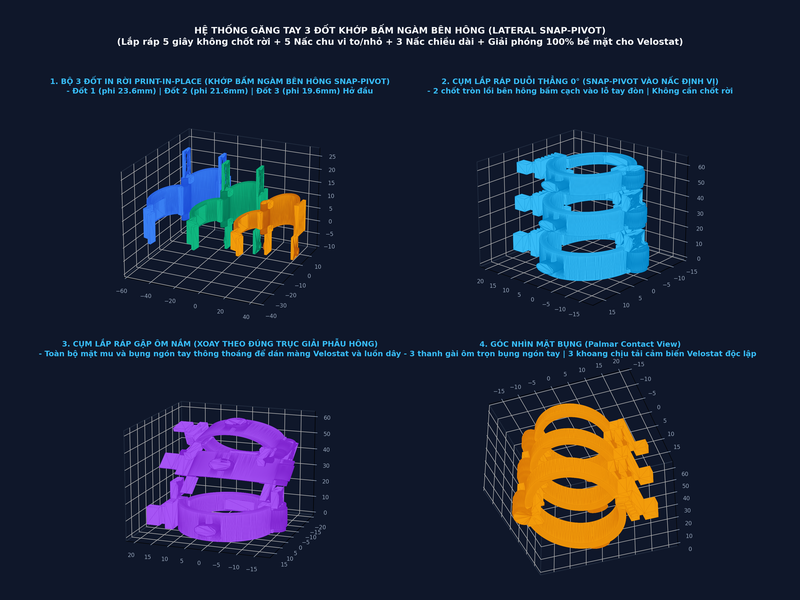
\includegraphics[width=4.4cm, height=2.6cm, keepaspectratio]{assets/splint_3d.png}
};
\node[below=2pt of hand, align=center, font=\small\bfseries] (hand_lbl) {
  Bàn tay mang nẹp 3 ngón\\
  {\footnotesize (16 Velostat vi sai + 3 Flex)}
};

% 2. TRÊN CÙNG Ở GIỮA: CAMERA & DEPTH ANYTHING V2
\node (camera) at (0.2, 3.2) {
  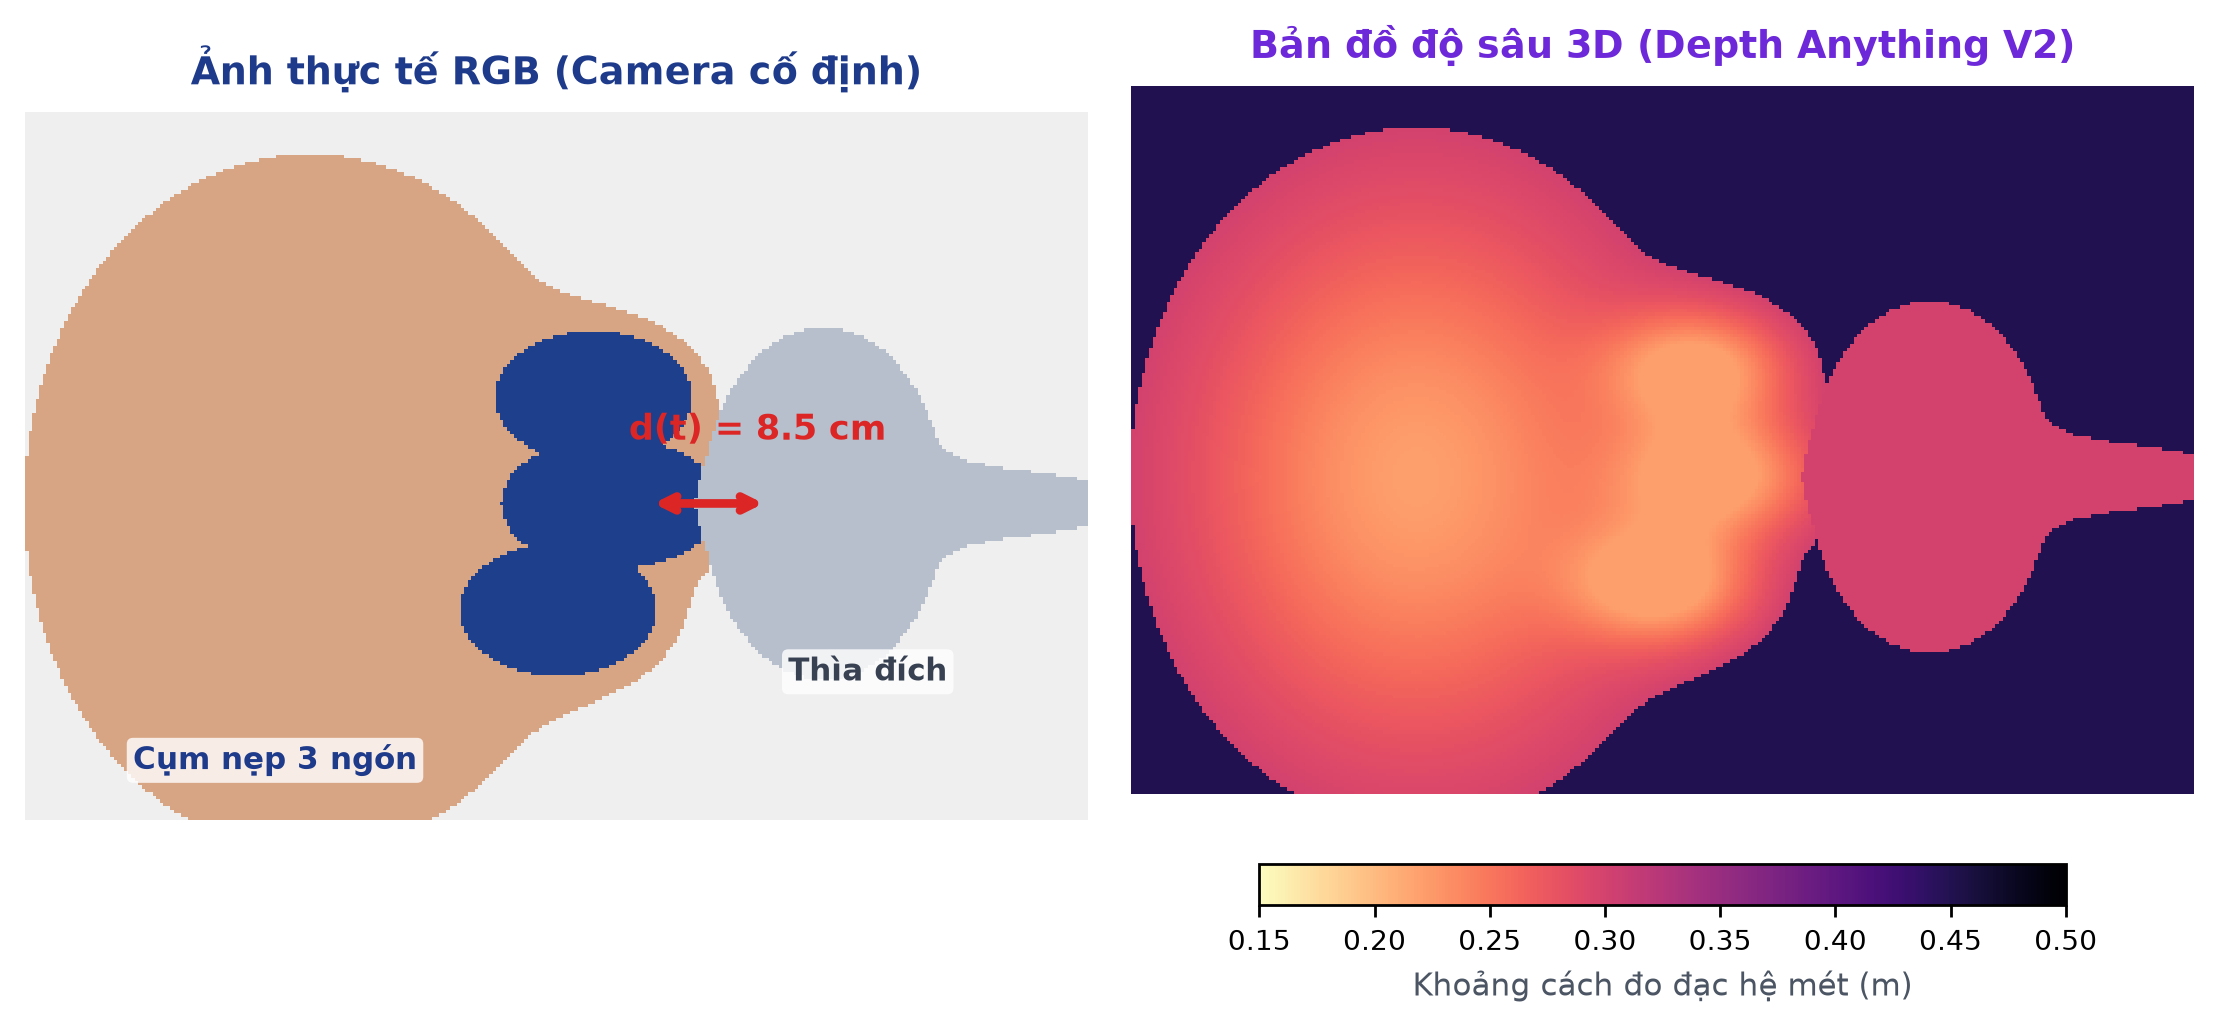
\includegraphics[width=5.8cm, height=2.4cm, keepaspectratio]{assets/depth_anything_scene.png}
};
\node[below=2pt of camera, align=center, font=\small\bfseries] (camera_lbl) {
  Camera RGB \& Depth Anything V2\\
  {\footnotesize (Ước lượng độ sâu 3D \& Định thời TTC)}
};

% 3. GÓC TRÊN BÊN PHẢI: KHUNG ĐIỀU KHIỂN ESP32-S3
\node[dashedBox, text width=4.8cm] (ctrl) at (6.0, 3.2) {
  {\bfseries\normalsize Bộ điều khiển}\\[4pt]
  \begin{tikzpicture}
    \node[draw=black, dashed, line width=0.8pt, fill=white, rounded corners=3pt, inner sep=3pt] (ads) at (-1.1, 0) {
      {\scriptsize\bfseries ADS1115 (16-bit)}
    };
    \node[draw=black, dashed, line width=0.8pt, fill=white, rounded corners=3pt, inner sep=3pt] (dsp) at (1.1, 0) {
      {\scriptsize\bfseries Thuật toán AAN}
    };
  \end{tikzpicture}\\[4pt]
  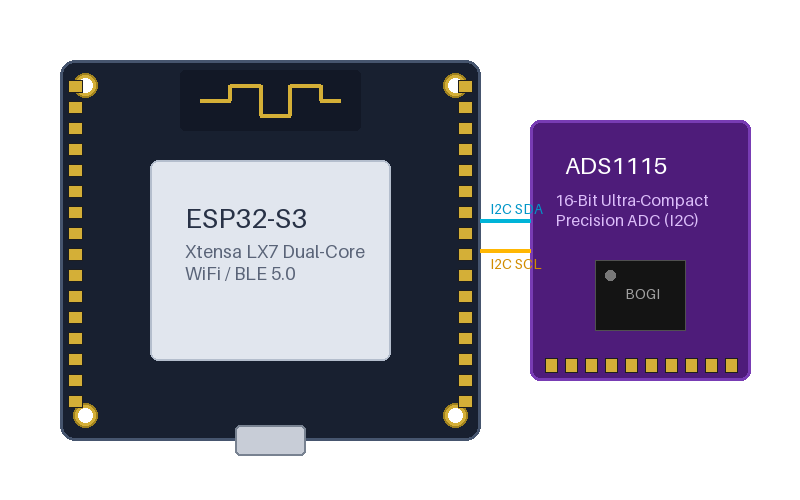
\includegraphics[width=4.2cm, height=1.6cm, keepaspectratio]{assets/controller_ads_board.png}\\[2pt]
  {\footnotesize Vi điều khiển ESP32-S3 (DSP 2 nhánh)}
};
\node[below=2pt of ctrl, align=center, font=\small\bfseries] {Xử lý tín hiệu \& Tính EI -- GAP -- RAL};

% 4. GÓC DƯỚI BÊN PHẢI: TRỢ LỰC SERVO & TANG CÁP
\node (act) at (6.0, -2.5) {
  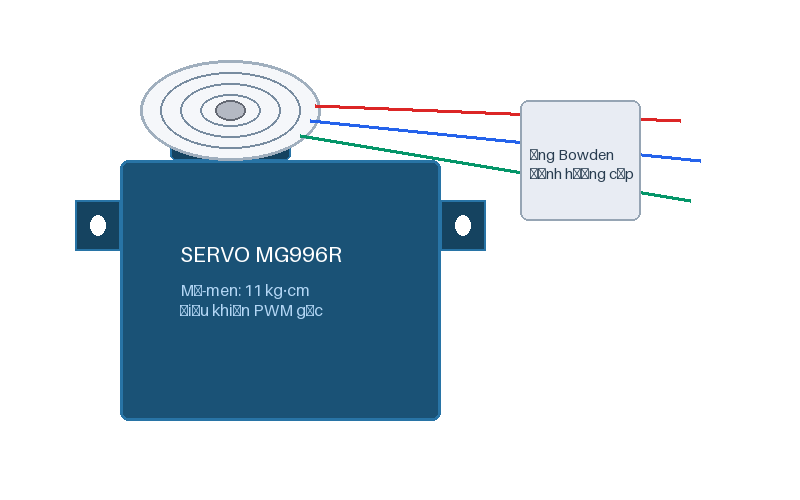
\includegraphics[width=4.8cm, height=2.4cm, keepaspectratio]{assets/servo_spool_assembly.png}
};
\node[below=2pt of act, align=center, font=\small\bfseries] (act_lbl) {
  Cụm 3 Servo MG996R \& Tang cuốn cáp\\
  {\footnotesize (Kéo gập chủ động / Nhả cáp duỗi)}
};

% 5. MŨI TÊN LIÊN KẾT VÒNG LẶP KHÉP KÍN (Chuẩn như sơ đồ xe lăn điều khiển mắt)
% Từ Tay -> Camera (Camera theo dõi cự ly tay)
\draw[arrowMain] (hand.east) -- node[tagLbl, above=2pt] {Quan sát cự ly 3D} (camera.west);

% Từ Camera -> ESP32-S3 (Khẩu độ đón trước & TTC)
\draw[arrowMain] (camera.east) -- node[tagLbl, above=2pt] {Khẩu độ \& TTC} (ctrl.west);

% Từ Cảm biến trên nẹp -> chạy thẳng sang ESP32-S3 (đường phía trên uốn cong nhẹ hoặc thẳng)
\draw[arrowMain] (hand.north) -- ++(0, 0.8cm) -| node[tagLbl, pos=0.25, above=2pt] {Tín hiệu cảm biến: Lực tiếp xúc \& Góc gập ngón} (ctrl.north);

% Từ ESP32-S3 đi xuống Servo
\draw[arrowMain] (ctrl.south) -- node[tagLbl, right=3pt] {Lệnh servo AAN} (act.north);

% Từ Servo quay về Bàn tay mang nẹp (Đường ngang dưới khép kín vòng lặp)
\draw[arrowMain] (act.west) -| node[tagLbl, pos=0.25, below=3pt] {Cáp Bowden kéo trợ lực gập ngón / Nhả duỗi mở khẩu độ} (hand_lbl.south);

\end{tikzpicture}
\end{document}
